% !TEX root = ../vr_st.tex

\section{Barcode estimates}\label{s:computations}

\subsection{Barcode estimates}\label{sub:general_barcodes}

We estimate the barcodes of $\R$-spaces in terms of their \textit{first critical values}.

\subsubsection{}\label{subsub:first_critical_value}

Let $X$ be an $\R$-space which is empty for negative numbers, with the Vietoris--Rips complex of a metric space as a primary example.
From now on, we will consider this $\R$-space and omit it from the notation when convenient.
Its \defn{first critical value} is the supremum among real numbers $r$ such that $X_{s,t}$ is a homotopy equivalence for any $s,t \in [0,r]$.

The \defn{first critical value} of a persistent module which is \(0\) for negative numbers is defined analogously.

\medskip\remark
Clearly, the first critical value of an $\R$-space is bounded above by the first critical value of its $\degp^\th$ homology, as well as that of any $\theta$-barcode for $\theta$ a linear cohomology operation.

\subsubsection{}\label{subsub:barcode_general}

Let \(\degp \in \N\) and \(\theta \in \cO(\ell,\degp)\) a linear cohomology operation with \(\ell \neq \degp\).
We respectively denote by $\alpha, \beta_\degp$ and $\gamma_\degp$ the first critical values of $X$, \(\rH_\degp\), and \(\img_\theta\).

Because the $\R$-space $X$ begins at $r=0$ and the homotopy type of $X_r$ remains unchanged for $r\in [0,\alpha)$, bars in both the homology barcodes and the $\theta$-barcodes either start at $0$ or start after $\alpha$.

In addition, for degrees $\degp$ such that $\rH_\degp(X_0)$ is non-trivial, the barcode of the $\degp^\th$ reduced homology of $X$ always contains $(0,\beta_\degp )$.
For linear cohomology operations $\theta \in \cO(\ell, \degp)$ such that $\img \theta_{X_0}$ is non-trivial, the $\theta$-barcode of $X$ always contains $(0,\gamma_\degp)$.
\anibal{The fact that the maps are not isomorphisms after their critical value does not imply that they are not injective. You can say that they contain a bar dominated by \((0,\gamma_\degp)\)}.
We illustrate our estimate of the barcodes of $X$ in \cref{fig:barcodes_general}\anibal{Why are there 3 dots on the left?}.

\begin{figure}
	\centering
	\begin{tikzpicture}[scale=0.52]
	\begin{axis} [
		title = {\LARGE $\barc\opH_m^{\VR}(\cM)$, if $\opH_m(\cM) \neq 0$},
		ticklabel style = {font=\Large},
		axis y line=middle,
		axis x line=middle,
		ytick={0.7,0.95},
		yticklabels={$2\firstdeath{m}{\cM}$,$\diam(\cM)$},
		xtick={0.55,0.95},
		xticklabels={$2\crit(\cM)$, $\diam(\cM)$},
		xmin=-0.015, xmax=1.1,
		ymin=0, ymax=1.1,]
		\addplot [mark=none] coordinates {(0,0) (1,1)};
		\addplot [thick,color=black!20!white,fill=black!30!white,
		fill opacity=0.4]coordinates {
			(0.55,0.95)
			(0.55,0.55)
			(0.95,0.95)
			(0.55,0.95)};
		\addplot [black!40!white,mark=none,dashed, thin] coordinates {(0,0.7) (0.7,0.7)};
		\addplot [black!40!white,mark=none,dashed, thin] coordinates {(0,0.55) (0.55,0.55)};
		\addplot [black!40!white,mark=none,dashed, thin] coordinates {(0.55,0) (0.55,0.55)};
		\addplot[line width=1.5mm, color=black!30!white] coordinates{(0, 0.7) (0, 0.95)};
		\addplot[barccolor,mark=*] (0, 0.7) circle (2pt) node[above right,barccolor]{};
	\end{axis}
\end{tikzpicture}
\begin{tikzpicture}[scale=0.52]
	\begin{axis} [
		title = {\LARGE $\barc\opH_m^{\VR}(\cM)$, if $\opH_m(\cM) = 0$},
		ticklabel style = {font=\Large},
		axis y line=middle,
		axis x line=middle,
		ytick={0.95},
		yticklabels={$\diam(\cM)$},
		xtick={0.55,0.95},
		xticklabels={$2\crit(\cM)$, $\diam(\cM)$},
		xmin=-0.015, xmax=1.1,
		ymin=0, ymax=1.1,]
		\addplot [mark=none] coordinates {(0,0) (1,1)};
		\addplot [thick,color=black!20!white,fill=black!30!white,
		fill opacity=0.4]coordinates {
			(0.55,0.95)
			(0.55,0.55)
			(0.95,0.95)
			(0.55,0.95)};
		\addplot [black!40!white,mark=none,dashed, thin] coordinates {(0,0.55) (0.55,0.55)};
		\addplot [black!40!white,mark=none,dashed, thin] coordinates {(0.55,0) (0.55,0.55)};
	\end{axis}
\end{tikzpicture}

\begin{tikzpicture}[scale=0.52]
	\begin{axis} [
		title={\LARGE $\thetabarc{\cM}$, if $\img\theta_{\cM}\neq 0$},
		ticklabel style = {font=\Large},
		axis y line=middle,
		axis x line=middle,
		ytick={0.7,0.95},
		yticklabels={$2\firstdeath{\theta}{\cM}$,$\diam(\cM)$},
		xtick={0.55,0.95},
		xticklabels={$2\crit(\cM)$, $\diam(\cM)$},
		xmin=-0.015, xmax=1.1,
		ymin=0, ymax=1.1,]
		\addplot [mark=none] coordinates {(0,0) (1,1)};
		\addplot [thick,color=black!20!white,fill=black!30!white,
		fill opacity=0.4]coordinates {
			(0.55,0.95)
			(0.55,0.55)
			(0.95,0.95)
			(0.55,0.95)};
		\addplot [black!40!white,mark=none,dashed, thin] coordinates {(0,0.7) (0.7,0.7)};
		\addplot [black!40!white,mark=none,dashed, thin] coordinates {(0,0.55) (0.55,0.55)};
		\addplot [black!40!white,mark=none,dashed, thin] coordinates {(0.55,0) (0.55,0.55)};
		\addplot[line width=1.5mm, color=black!30!white] coordinates{(0, 0.7) (0, 0.95)};
		\addplot[barccolor,mark=*] (0, 0.7) circle (2pt) node[above right,barccolor]{};
	\end{axis}
\end{tikzpicture}
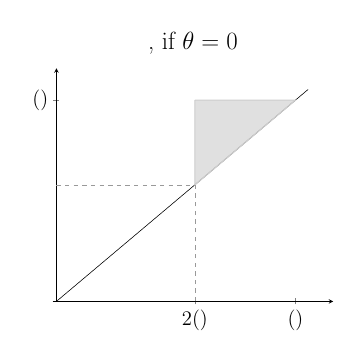
\begin{tikzpicture}[scale=0.52]
	\begin{axis} [
		title={\LARGE $\thetabarc{\cM}$, if $\img\theta_{\cM}= 0$},
		ticklabel style = {font=\Large},
		axis y line=middle,
		axis x line=middle,
		ytick={0.95},
		yticklabels={$\diam(\cM)$},
		xtick={0.55,0.95},
		xticklabels={$2\crit(\cM)$, $\diam(\cM)$},
		xmin=-0.015, xmax=1.1,
		ymin=0, ymax=1.1,]
		\addplot [mark=none] coordinates {(0,0) (1,1)};
		\addplot [thick,color=black!20!white,fill=black!30!white,
		fill opacity=0.4]coordinates {
			(0.55,0.95)
			(0.55,0.55)
			(0.95,0.95)
			(0.55,0.95)};
		\addplot [black!40!white,mark=none,dashed, thin] coordinates {(0,0.55) (0.55,0.55)};
		\addplot [black!40!white,mark=none,dashed, thin] coordinates {(0.55,0) (0.55,0.55)};
	\end{axis}
\end{tikzpicture}
	\caption{Let $X$ be an $\R$-space where $X_r$ is empty for $r<0$ and contractible for $r\geq R$ for some real number $R$. \emph{Top row:} the $\degp^\th$ persistent homology barcode of $X$; the leftmost one contains one $(0,\beta_m)$ and some bars of the form $(0,a)$ for some $a\in [\beta_\degp, R]$.
		\emph{Bottom row:} $\theta$-barcodes of $X$, where $\theta\in\cO(\ell,\degp)$ is a linear cohomology operation; the leftmost one contains one $(0,\gamma_m)$ and some bars of the form $(0,b)$ for some $b\in [\beta_\degp, R]$.}
	\label{fig:barcodes_general}
\end{figure}

\subsection{$n$-sphere}\label{ss:Sn}

For any integer $n \geq 1$ and real number $r > 0$, let $\bS^n(r)$ be the \defn{$n$-sphere} of radius $r$ centered at the origin of $\R^{n+1}$.
We consider it equipped with the geodesic distance.
We simplify notation writing \(\bS^n\) instead of \(\bS^n(1)\).

Because the Vietoris--Rips complexes of $\bS^n$ is contractible when the scale parameter is greater than $\pi$, all its bars are dominated by $(0, \pi)$.

Recall from \cite[Thm.~7.1]{lim2020vietoris} that for $n \in \N$ and
\[
0 < r \leq \zeta_n \defeq \arccos(\tfrac{-1}{n+1}),
\]
the space $\VR_r\bS^n$ is homotopy equivalent to $\bS^n$.
This implies that, for any degree~$\degp$, all bars in $\barc\rH_\degp (\VR\bS^n)$ are dominated by $(\zeta_n,\pi)$ with the exception of a single bar $(0,\zeta_n)$ when $d = n$ (see Figure \ref{fig:Sk}).\footnote{
	The case $n = 1$ has more information.
	From \cite[Thm.~7.4]{adamaszek2017vietoris} it is known that $\VR_r\bS^1$ is homotopy equivalent to $\bS^{2n+1}$ for any $n \in \N$ and $\frac{2n\pi}{2n+1} < r \leq \frac{2(n+1)\pi}{2n+3}$.
	For $d=1$ and $n > 1$ and one also has more information.
	Recall that a metric space $(\cX, d)$ is said to be a \defn{geodesic space} if for each $x, y \in \cX$ there exists geodesic from $x$ to $y$ of length $d(x, y)$.
	As stated in \cite[Prop.~7.10]{virk20201} one knows that if $\cX$ be a simply-connected geodesic space, then $\barc\rH_1(\cX) = \emptyset$.
	Since the spheres we are considering are geodesic their $\rH_1$ barcode is empty. \ling{We may simplify the footnote.}}

\begin{figure}[ht]
	\centering
	\begin{tabular}{ c c }
	\begin{tikzpicture}[scale=0.6]
		\begin{axis} [
			title = {\LARGE $\barc\rH_n(\bS^n)$},
			ticklabel style = {font=\Large},
			axis y line=middle,
			axis x line=middle,
			ytick={0.5,0.57,0.67,0.95},
			yticklabels={,$\zeta_n$,,$\pi$},
			xtick={0.5,0.57,0.95},
			xticklabels={$\frac{\pi}{2}$,$\zeta_n$, $\pi$},
			xmin=-0.015, xmax=1.1,
			ymin=0, ymax=1.1,]
			\addplot [thick,color=black!20!white,fill=black!30!white,
			fill opacity=0.4]coordinates {
				(0.57,0.95)
				(0.57,0.57)
				(0.95,0.95)
				(0.57,0.95)};
			\addplot [black!40!white,mark=none,dashed, thin] coordinates {(0,0.57) (0.57,0.57)};
			\addplot [black!40!white,mark=none,dashed, thin] coordinates {(0.57,0) (0.57,0.57)};
			\addplot[barccolor,mark=*] (0, 0.57) circle (2pt) node[above right,barccolor]{};{\Large\textsf{1}};
			\addplot [mark=none] coordinates {(0,0) (1,1)};
		\end{axis}
	\end{tikzpicture}
	&
	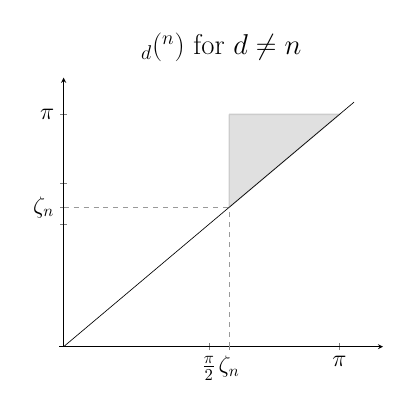
\begin{tikzpicture}[scale=0.6]
		\begin{axis} [
			title = {\LARGE $\barc\rH_d(\bS^n)$ for $d \neq n$},
			ticklabel style = {font=\Large},
			axis y line=middle,
			axis x line=middle,
			ytick={0.5,0.57,0.67,0.95},
			yticklabels={,$\zeta_n$,,$\pi$},
			xtick={0.5,0.57,0.95},
			xticklabels={$\frac{\pi}{2}$,$\zeta_n$, $\pi$},
			xmin=-0.015, xmax=1.1,
			ymin=0, ymax=1.1,]
			\addplot [thick,color=black!20!white,fill=black!30!white,
			fill opacity=0.4]coordinates {
				(0.57,0.95)
				(0.57,0.57)
				(0.95,0.95)
				(0.57,0.95)};
			\addplot [black!40!white,mark=none,dashed, thin] coordinates {(0,0.57) (0.57,0.57)};
			\addplot [black!40!white,mark=none,dashed, thin] coordinates {(0.57,0) (0.57,0.57)};
			\addplot [mark=none] coordinates {(0,0) (1,1)};
		\end{axis}
	\end{tikzpicture}
\end{tabular}
	\caption{Estimation of the persistent homology barcode of $\bS^n$.
	In each figure, the gray area represents the only region, apart from the blue dot, where points could potentially exist within the corresponding barcode.
	Here, and throughout the paper, $\zeta_n = \arccos(\tfrac{-1}{n+1})$ and $\rH_\degp $ denotes reduced $\degp$-homology.
	We remark that for any \(n \in \N\) the value \(\zeta_n\) is bounded below by \(\pi/2\).}
	\label{fig:Sk}
\end{figure}

Similarly, for any linear cohomology operation $\theta \in \cO(\ell,m)$ with $\ell \neq m$, every bar in the barcode of $\img\theta_{\VR\bS^n}$ or $\ker\theta_{\VR\bS^n}$ is dominated by $(\zeta_n,\pi)$.

\subsection{Wedge sum of spheres}

\subsubsection{}

For $n \in \N$ and $\ell_1, \dots, \ell_n \in \N^n$, let
\[
\VS^{\ell_1,\dots,\ell_n} =
\overbrace{\bS^1\vee\dots\vee\bS^1}^{\ell_1} \vee\dots\vee \overbrace{\bS^n\vee\dots\vee\bS^n}^{\ell_n}.
%(\bS^1)^{\vee m_1} \vee \dots \vee (\bS^n)^{\vee m_n}.
\]
Using the homotopy equivalence between the Vietoris--Rips filtration of a metric gluing with the wedge sum of the Vietoris--Rips filtration described in \cref{ss:wedge sum}, we have the following isomorphisms of persistence modules:
\[
\rH_\degp (\VR\VS^{\ell_1,\dots,\ell_n}) \cong \, \bigoplus_{i=1}^n \rH_\degp (\VR\bS^i)^{\oplus \ell_i}
\]
for any \(m \in \N\) and
\[
\img\theta_{\VR(\VS^{\ell_1,\dots,\ell_n})} \cong \, \bigoplus_{i=1}^n (\img\theta_{\VR\bS^i})^{\oplus \ell_i}
\]
for any linear cohomology operation.
Therefore, the barcode of $\rH_\degp(\VS^{\ell_1,\dots,\ell_n})$ contains $\ell_\degp$ copies of $(0,\zeta_\degp)$.
All remaining bars in this barcode must be dominated by $(\zeta_n, \pi)$.
This holds for all degrees, with the convention that $\ell_\degp = 0$ for $\degp > n$.

Similarly, for any linear cohomology operation $\theta \in \cO(\ell,m)$ with $\ell \neq m$, every bar in either its $\img\theta$ or $\ker\theta$ barcode is dominated by $(\zeta_n, \pi)$.

\begin{figure}
	\centering
	\begin{tikzpicture}[scale=0.52]
	\begin{axis} [
		title = {\LARGE $\Hbarc[\field]{\degp}{\VS^n},1\leq \degp\leq n$},
		ticklabel style = {font=\Large},
		axis y line=middle,
		axis x line=middle,
		ytick={0.5,0.6,0.67,0.95},
		yticklabels={,$\zeta_\degp$,,$\pi$},
		xtick={0.5,0.55,0.95},
		xticklabels={$\frac{\pi}{2}$,$\zeta_n$, $\pi$},
		xmin=-0.015, xmax=1.1,
		ymin=0, ymax=1.1,]
		\addplot [mark=none] coordinates {(0,0) (1,1)};
		\addplot [thick,color=black!20!white,fill=black!30!white,
		fill opacity=0.4]coordinates {
			(0.55,0.95)
			(0.55,0.55)
			(0.95,0.95)
			(0.55,0.95)};
		\addplot [black!40!white,mark=none,dashed, thin] coordinates {(0,0.6) (0.6,0.6)};
		\addplot [black!40!white,mark=none,dashed, thin] coordinates {(0,0.55) (0.55,0.55)};
		\addplot [black!40!white,mark=none,dashed, thin] coordinates {(0.55,0) (0.55,0.55)};
		\addplot[barccolor,mark=*] (0, 0.6) circle (2pt) node[above right,barccolor]{};%{\Large\textsf{1}};
		%\node[mark=none] at (axis cs:0.68,0.21){$\Hbarc{2}{\VS^n}$};
	\end{axis}
\end{tikzpicture}
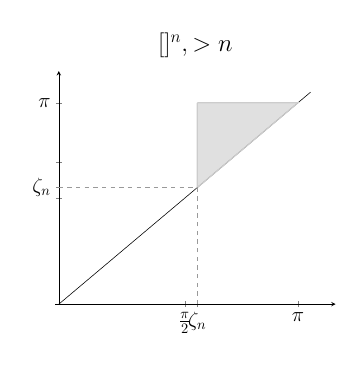
\begin{tikzpicture}[scale=0.52]
	\begin{axis} [
		title = {\LARGE $\Hbarc[\field]{\degp}{\VS^n}, \degp>n$},
		ticklabel style = {font=\Large},
		axis y line=middle,
		axis x line=middle,
		ytick={0.5,0.55,0.67,0.95},
		yticklabels={,$\zeta_n$,,$\pi$},
		xtick={0.5,0.55,0.95},
		xticklabels={$\frac{\pi}{2}$,$\zeta_n$, $\pi$},
		xmin=-0.015, xmax=1.1,
		ymin=0, ymax=1.1,]
		\addplot [mark=none] coordinates {(0,0) (1,1)};
		\addplot [thick,color=black!20!white,fill=black!30!white,
		fill opacity=0.4]coordinates {
			(0.55,0.95)
			(0.55,0.55)
			(0.95,0.95)
			(0.55,0.95)};
		\addplot [black!40!white,mark=none,dashed, thin] coordinates {(0,0.55) (0.55,0.55)};
		\addplot [black!40!white,mark=none,dashed, thin] coordinates {(0.55,0) (0.55,0.55)};
		%\node[mark=none] at (axis cs:0.68,0.21){$\Hbarc[\field]{\degp}{\VS^n}, \degp\geq 3$};
	\end{axis}
\end{tikzpicture}

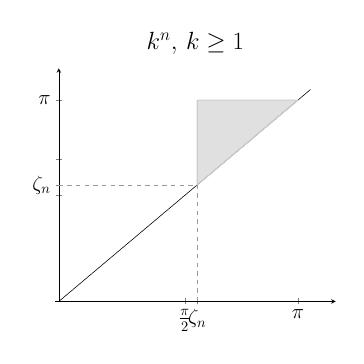
\begin{tikzpicture}[scale=0.52]
	\begin{axis} [
		title={\LARGE $\sqbarc{k}{\VS^n},\, k\geq 1$},
		ticklabel style = {font=\Large},
		axis y line=middle,
		axis x line=middle,
		ytick={0.5,0.55,0.67,0.95},
		yticklabels={,$\zeta_n$,,$\pi$},
		xtick={0.5,0.55,0.95},
		xticklabels={$\frac{\pi}{2}$,$\zeta_n$, $\pi$},
		xmin=-0.015, xmax=1.1,
		ymin=0, ymax=1.1,]
		\addplot [mark=none] coordinates {(0,0) (1,1)};
		\addplot [thick,color=black!20!white,fill=black!30!white,
		fill opacity=0.4]coordinates {
			(0.55,0.95)
			(0.55,0.55)
			(0.95,0.95)
			(0.55,0.95)};
		\addplot [black!40!white,mark=none,dashed, thin] coordinates {(0,0.55) (0.55,0.55)};
		\addplot [black!40!white,mark=none,dashed, thin] coordinates {(0.55,0) (0.55,0.55)};
		%\node[mark=none] at (axis cs:0.68,0.21){$\sqbarc{k}{\VS^n},\, k\geq 1$};
	\end{axis}
\end{tikzpicture}

	\caption{Let $\VS\defeq \VS^{\ell_1,\dots,\ell_n}$.
	\emph{Top row:} persistent homology barcodes of $\VS$, where the dot $(0,\zeta_m)$ has multiplicity $\ell_m$.
	\emph{Bottom row:} $\theta$-barcodes of $\VS$ where $\theta \in \cO(\ell,m)$ is any linear cohomology operation with \(\ell \neq m\).}
	\label{fig:barcodes_vs}
\end{figure}

\subsection{First critical values of $\rp^n$}\label{sub:first_critical_value_rpn}

\subsubsection{}

We will consider the following metric model of the \defn{real projective $n$-space}.
Let $\rp^n(r)$ be the quotient space $\bS^n(r)$ by the antipodal map $x \mapsto -x$ for all $x \in \bS^n$.
We equip $\rp^n(r)$ with the quotient metric:
\[
d\big([x],[x']\big) =
\min\set[\big]{d(x, x'), d(-x, x')}.
\]
To simplify notation we denote $\rp^n(2)$ by $\rp^n$ noticing that
\[
\diam(\bS^n) = \diam(\rp^n) = \pi.
\]

\subsubsection{}

Let \(\alpha\) denote the first critical value of \(\VR\rp^n\).
From \cite[Thm.~4.5]{adams2022metric} we have the following.

\medskip\proposition
The first critical value of \(\VR\rp^n\) is \(\alpha = \frac{2\pi}{3}\).
%
%for $r \in (0,\frac{2\pi}{3}]$
%\[
%\VR_r(\rp^n) \simeq \rp^n.
%\]


%For \(\degp \in \N\) we denote by \(\beta_\degp\) the first critical value of its \(\degp^\th\) reduced homology with mod 2 coefficients, and \(\gamma_{\ell+\degp}\)


%, consider the cohomology operations to be the Steenrod squares.
%Let $\alpha, \beta_\degp$ and $\gamma_\degp$ denote the first critical values of $\VR\rp^n$, the $\degp^\th$ reduced homology of $\VR\rp^n$ with mod two coefficients and the degree-$\degp$ component of the Steenrod barcode of $\VR\rp^n$, respectively.
%
%It follows from \cref{prop:homotopy type} that $\alpha = \frac{2\pi}{3}$.
%For the values of $\beta_\degp$ and $\gamma_\degp$, see \cref{subsub:beta_m_rpn} and \cref{subsub:gamma_rpn}, respectively.

\subsubsection{}\label{subsub:gamma_rpn}

Let us now consider the mod-\(2\) cohomology of \(\VR\rp^n\) and the linear cohomology operations defined by Steenrod squares \(\Sq^k_\ell \in \cO(\ell,\ell+k)\).
Denoting by \(\gamma_{\ell+k}\) the first critical value of \(\img_{\Sq^k_\ell}\) on \(\VR\rp^n\) we have the following.

\medskip\proposition
If $k,\ell$ are positive integers such that $k \leq \min\{\frac{n-1}{2}, \ell\} \leq n$ and $\binom{\ell}{k}$ is odd, then $\gamma_{k+\ell} = \tfrac{2\pi}{3}$.

\begin{proof}
	Since the Vietoris--Rips complex $\VR_r\rp^n$ retains the homotopy type of $\rp^n$ for $r \in [0,\tfrac{2\pi}{3})$, $\Sq^k(\alpha^\ell) = \binom{\ell}{k}\alpha^{\ell+k}$ generates a bar in the $\Sq^k_\ell$--barcode that is born at $0$ and stay alive until the non-trivial degree-$(\ell+k)$ class $\alpha^{k+\ell}$ dies at $\tfrac{2\pi}{3}$.
	Thus, the first critical value of $\gamma_{k+\ell} \leq \tfrac{2\pi}{3}$.
	On the other hand, $\gamma_{k+\ell} \geq \alpha = \tfrac{2\pi}{3}$ the first critical value of $\VR\rp^n$.
	Thus, $\gamma_{k+\ell} = \tfrac{2\pi}{3}$.
	\anibal{We do not know that it dies.}
\end{proof}

\subsubsection{}\label{subsub:beta_m_rpn}

We devote the remaining part of \cref{sub:general_barcodes} to prove the following proposition about the first critical value of the homology of $\VR\rp^n$.

\medskip\proposition
$\beta_m=\frac{2\pi}{3}$ for any $1\leq m\leq n$.

\subsubsection{}\label{subsub:h}

We begin by examining the relationship between the Vietoris--Rips filtration of a quotient space and the Vietoris--Rips filtration induced by the quotient.
The following proposition is proved in \cite[Proposition 3.5]{adams2022metric}, we include a proof sketch below for clarity.

\medskip\lemma
Let $G$ acts properly and by isometry on $\cX$, and the action of $G$ on $\cX$ is a $r^*$-diameter action for $r>0$. Then, the map
\[
h \colon \VR_r\cX_G \to (\VR_r\cX)_G
\text{ with }
\sum_{i=1}^k \lambda_i [x_i] \mapsto [\sum_{i=1}^k \lambda_i x_i]
\]
is an isomorphism of simplicial complexes.

\begin{proof}
	Because $G$ acts by isometry, we have a well-defined map
	\[
	\tilde{h} \colon \VR_r\cX \to \VR_r\cX_G
	\text{ with }
	\sum_{i=1}^k \lambda_i x_i \mapsto \sum_{i=1}^k \lambda_i [x_i],
	\]
	Because two points in the same orbit of the $G$ action always have the same image under $\tilde{h}$, it induces a map $\tilde{h}_G \colon (\VR_r\cX)_G \to \VR_r\cX_G$.

	Moreover, $\tilde{h}_G$ is an isomorphism, following from the fact that the action of $G$ on $\cX$ is an $r^*$-diameter action; see \cite[Proposition 3.5]{adams2022metric} for further details.
	Therefore, $h$, the inverse of $\tilde{h}_G$, is also an isomorphism.
\end{proof}

\subsubsection{}
\label{subsub:f}

For any $r<\pi$, let $f$ be the composition
\[
f \colon \VR_r\bS^n \to \R^{n+1} \setminus \set{0} \xra{\pi} \bS^n,
\]
where the first map sends a formal linear sum $\sum_{i=1}^k \lambda_i x_i$ in the Vietoris--Rips thickening $\VR_r\bS^n$ to the point $\sum_{i=1}^k \lambda_i x_i \in \bbR^{n+1}$ where $x_i \in \bS^n$ and $\lambda_i \in [0,1]$ satisfying $\sum_i\lambda_i=1$, and the second map $\pi$ is the radial projection map.

\medskip\lemma
When $0<r<\zeta_n=\arccos{(-\tfrac{1}{n+1})}$, the map $f$ is a weak homotopy equivalence.
\footnote{For $0<r<\zeta_n$, the Vietoris-Rips complex $\VR_r\bS^n$ is indeed homotopic to $\bS^n$, as shown in \cite[Theorem 7.1]{lim2020vietoris}.}

\begin{proof}
	To prove the statement, we use an intermediate construction called the Vietoris--Rips thickening, introduced in \cite{adamaszek2018metric} as a metric space analogue of the Vietoris--Rips complexes.

	The Vietoris--Rips thickening $\VR_r^m\cX$ of a metric space $\cX$ at a given scale $r$ is defined as the set of convex linear combinations of the Dirac probability measures $\delta_{x}$ on points $x \in X$, equipped with the $1$-Wasserstein metric.
	There is a set bijection from $g \colon \VR_r\cX \to \VR_r^m\cX$, given by $\sum_{i=1}^k\lambda_i x_i\mapsto \sum_{i=1}^k\lambda_i\delta_{x_i}.$
	%As this object is not the center of the discussion here, we omit the details and only state the related results here.
	It is shown in \cite[Theorem 1]{gillespie2024vietoris} that (for open Vietoris-Rips complexes) the natural bijection $g$ is a weak homotopy equivalence.

	In the case of $\cX = \bS^n$, the map $f$ is the composition of two maps
	\[\VR_r\bS^n\xrightarrow{g}\VR_r^m\bS^n\xrightarrow{f \circ g^{-1}}\bS^n.\]
	According to \cite[Proposition 5.3]{adamaszek2018metric}, when $0<r<\zeta_n$, $f \circ g^{-1}$ is a homotopy equivalence, implying that $f = (f \circ g^{-1}) \circ g$ is a weak homotopy equivalence.
\end{proof}

\subsubsection{}
\label{subsub:rho}
Let $f$ be the map defined in \cref{subsub:f}.
Let $G$ be a group action on $\bS^n$ that commutes with $f$.
Let $f_G \colon \VR_r\bS^n_G \to \bS^n_G$ be the induced map of $f$.

\medskip\lemma
For any $0<r<\zeta_n$, the following composition is a weak homotopy equivalence
\[
\rho \defeq h \circ f_G
\colon \VR_r\bS^n_G \to \bS^n_G.
\]
\begin{proof}
	By \cref{subsub:f}, the map $f$ is a weak homotopy equivalence when $0<r<\zeta_n$.
	Then, because $G$ is a group action on $\bS^n$ preserved by $f$, the induced map $f_G$ is also a weak homotopy equivalence.
	Furthermore, as the map $h$ (defined in \cref{subsub:h}) is a homomorphism, its composition with $f_G$ is a weak homotopy equivalence.
\end{proof}

\subsubsection{}

Let $\rho^n$ (or $\rho^{n-1}$) be the weak homotopy equivalence defined in \cref{subsub:rho} for the case of $\bS^n$ (or $\bS^{n-1}$).

\medskip\lemma
For $0<t\leq s $, we have the following diagram of topological spaces:
\begin{equation}\label{d:fundamental_bars_diagram}
	\begin{tikzcd}
		\bS^{n-1}_G
		\ar[d, hook,"{\iota}" left]
		&
		\VR_t\bS^{n-1}_G
		\ar[d, hook,"\iota_t"]
		\ar[l, "\rho^{n-1}" above]
		\ar[r, hook, "v^{n-1}"]
		&
		\VR_{s}\bS^{n-1}_G
		\ar[d, hook]
		\\
		\bS^{n}_G
		&
		\VR_t(\bS^{n}_G)
		\ar[l, "\rho^n" below]
		\ar[r, hook, "v^{n}"]
		&
		\VR_{s}\bS^{n}_G.
	\end{tikzcd}
\end{equation}
The horizontal inclusions $v^{n-1}$ and $v^n$ are induced by the Vietoris--Rips filtration.
The vertical maps are induced by the equatorial inclusion of real projective spaces $\iota \colon \bS^{n-1}_G \hookrightarrow \bS^{n}_G$.

\begin{proof}
	The commutativity of the right-hand-side square is straightforward.
	For the left-hand-side square, take any $y = \sum_{i=1}^k \lambda_i [x_i] \in \VR_t\bS^{n-1}_G$ and verify that
	\begin{center}
		$(\iota \circ \rho^{n-1})(y)
		=\iota(f^{n-1}_G([\sum_i \lambda_i x_i]))
		=\iota([f^{n-1}(\sum_i \lambda_i x_i)])
		=[\pi^{n-1}(\sum_i \lambda_i x_i)]
		$
	\end{center}
	as an element in $\bS^n_G$, and
	\begin{center}
		$(\rho^{n} \circ \iota_t)(y) = \rho^{n}(y) = f^{n}_G([\sum_i \lambda_i x_i]) = [f^{n}(\sum_{i=1}^k \lambda_i x_i)] = [\pi^{n}(\sum_i \lambda_i x_i)].
		$
	\end{center}
	Because $\pi^{n}$ restricted to $\bS^{n-1}_G$ is equal to $\pi^{n-1}$, we conclude that $(\iota \circ \rho^{n-1})(y) = (\rho^n \circ \iota_t)(y)$ for any $y$.
	Thus, the diagram commutes.
\end{proof}

\subsubsection{}
\label{subsub:foundamental_bar_rpn_lemma}

Let $\delta_n=2\mathrm{Fillrad}(\bS^n_G)$ and
let $\alpha_1$ be the first critical value of $\VR\bS^1_G$.
For any degree $1 \leq \degp \leq n$, let $\beta_{\degp, n}$ be the first critical value of the $\degp^\th$ reduced homology of $\VR(\bS^n_G)$.

\medskip\lemma
If $\delta_1 = \dots = \delta_n \leq \alpha_1$ and $\beta_{\degp, n} \leq \beta_{\degp, n'}$ for any $n\leq n'$, then
\[
\beta_{m, n} = \delta_1, \, \text{for any $1 \leq m \leq n$.}
\]

%We will refer to the bar in this lemma as the \defn{fundamental bar} of $\bS^n_G$.

\begin{proof}
	We will use an induction argument on $n$.
	When $n = 1$, it follows from \cref{ss:filling_radius} that
	\[
	(0, 2\mathrm{Fillrad}(\bS^1_G)) = (0, \delta_1) \in \Hbarc[\field]{1}{\bS^1_G}.
	\]
	This implies that $\rH_1(\VR\bS^1_G)$ changes isomorphism types at $\delta_1$, so $\beta_{1, 1} \leq \delta_1$.
	On the other hand, because $\delta_1 \leq \alpha_1$, $\rH_1(\VR\bS^1_G)$ retains the same isomorphism type before $\delta_1$, implying that $\beta_{1, 1} \geq \delta_1$.
	Thus, $\beta_{1, 1} =\delta_1$.

	Assume the statement holds for $\bS^{n-1}_G$, that is, $\beta_{m, n-1} = \delta_1$ for any $1\leq m \leq n-1$.
	Applying the $\degp^\th$ reduced homology functor to diagram \eqref{d:fundamental_bars_diagram}, we obtain the following commutative diagram of vector spaces:
	for $r,\epsilon>0$ small,
	\[
	\begin{tikzcd}
		\rH_\degp(\bS^{n-1}_G)
		\ar[d, "\cong" left]
		&
		\rH_\degp(\VR_r\bS^{n-1}_G)
		\ar[d, "\rH_\degp(\iota_r)" left, "\cong" right, myred]
		\ar[l, "\cong" above]
		\ar[rr, "\rH_\degp(v^{n-1})=0", myred]
		&
		&
		\rH_\degp(\VR_{\delta_1+\epsilon}\bS^{n-1}_G)
		\ar[d]
		\\
		\rH_\degp(\bS^{n}_G)
		&
		\rH_\degp(\VR_r(\bS^{n}_G))
		\ar[l, "\cong"]
		\ar[rr, "\rH_\degp(v^n)" , myred]
		&
		&
		\rH_\degp(\VR_{\delta_1+\epsilon}\bS^{n}_G).
	\end{tikzcd}
	\]
	Here, $\rH_\degp(f)$ for some map $f$ between topological spaces denotes the induced map of $f$ on the $\degp^\th$ reduced homology.

	Commutativity of the left-hand-side square implies that $\rH_\degp(\iota_r)$ is an isomorphism.
	By induction assumption, $\beta_{m, n-1} = \delta_1$ is the first critical value of $\rH_\degp(\VR\bS^{n-1}_G)$, which implies that $\rH_\degp(v^{n-1})$ is the zero map.
	Then, using the right-hand-side square's commutativity, we deduce $\rH_\degp(v^n) \circ \rH_\degp(\iota_r)=0$.
	Since $\rH_\degp(\iota_r)$ is an isomorphism, we conclude that $\rH_\degp(v^n)=0$.
	This holds for any $\epsilon>0$, so we can conclude $\beta_{m, n} \leq \delta_1$.
	On the other hand, we have $\delta_1 = \beta_{m, n-1} \leq \beta_{m, n}$.
	Therefore, $\beta_{m, n} = \delta_1$ holds for any $1\leq m \leq n-1$.

	For the case when $\degp=n$, we can apply \cref{ss:filling_radius} to obtain
	\[
	(0,2\mathrm{Fillrad}(\bS^n_G)) = (0, \delta_n) = (0, \delta_1) \in \Hbarc{n}{\bS^n_G}.
	\]

	Therefore, $(0, \delta_1) \in \Hbarc[\field]{\degp}{\bS^n_G}$ is established for all $1\leq \degp\leq n.$
\end{proof}

\subsubsection{}
We now prove the proposition in \cref{subsub:beta_m_rpn}.

\begin{proof}[Proof of \cref{subsub:beta_m_rpn}.]
	Recall that the filling radius of $\rp^n$ is $\frac{\pi}{3}$ for any $n \geq 1$.
	Therefore, \cref{ss:filling_radius} gives that $\delta_n = \tfrac{2\pi}{3} = \alpha_1$ for all $n$.
	Additionally, we have that
	\[
	\rp^1 \subset \rp^2 \subset \dots \subset \rp^n,
	\]
	with $\rp^\degp$ generating the $\degp^\th$ mod 2 homology of $\rp^n$ for every $1 \leq \degp \leq n$.
	This implies that $\beta_{\degp, n} \leq \beta_{\degp, n'}$ for any $n\leq n'$ and $\degp$.
	Applying \cref{subsub:foundamental_bar_rpn_lemma}, we obtain that $\beta_{m,n} = \delta_1 = \tfrac{2\pi}{3},$ for any $n\geq 1$ and $1 \leq m \leq n$.
\end{proof}

\subsection{Barcodes of $\rp^n$}\label{sub:barcode_rpn}

\anibal{This subsection is redundant if the subsection on barcode estimates is presented well. I placed it at the beginning of the section. Then the 3 examples will follow and use it to obtain the desired estimates.}

We have seen in \cref{sub:first_critical_value_rpn} that $\alpha = \beta_\degp = \gamma_{k+\ell} = \tfrac{2\pi}{3}$ for any $1 \leq \degp \leq n$ and $k, \ell$ such that $k \leq \frac{n-1}{2}$ s.t. $\binom{\ell}{k} \mod 2\neq 0$.

Applying \cref{subsub:barcode_general}, we obtain an estimate of the barcodes of $\rp^n$ and illustrate it in \cref{fig:sq barcodes}.

\begin{figure}
	\centering
	\begin{tikzpicture}[scale=0.52]
	\begin{axis} [
		title = {\LARGE $\Hbarc{\degp}{\rp^n},\, \degp\leq n$},
		ticklabel style = {font=\Large},
		axis y line=middle,
		axis x line=middle,
		ytick={0.5,0.67,0.95},
		yticklabels={$\frac{\pi}{2}$,$\frac{2\pi}{3}$,$\pi$},
		xtick={0.5,0.67,0.95},
		xticklabels={$\frac{\pi}{2}$,$\frac{2\pi}{3}$,$\pi$},
		xmin=-0.015, xmax=1.1,
		ymin=0, ymax=1.1,]
		\addplot [mark=none] coordinates {(0,0) (1,1)};
		\addplot [thick,color=black!20!white,fill=black!30!white,
		fill opacity=0.4]coordinates {
			(0.67,0.95)
			(0.67,0.67)
			(0.95,0.95)
			(0.67,0.95)};
		\addplot [black!40!white,mark=none,dashed, thin] coordinates {(0,0.67) (0.67,0.67)};
		%\addplot [black!40!white,mark=none,dashed, thin] coordinates {(0,0.72) (0.72,0.72)};
		\addplot [black!40!white,mark=none,dashed, thin] coordinates {(0.67,0) (0.67,0.67)};
		\addplot[barccolor,mark=*] (0, 0.67) circle (2pt) node[above right,barccolor]{};%{\Large\textsf{1}};
		%\node[mark=none] at (axis cs:0.68,0.21){$\Hbarc{1}{\rp^n}$};
	\end{axis}
\end{tikzpicture}
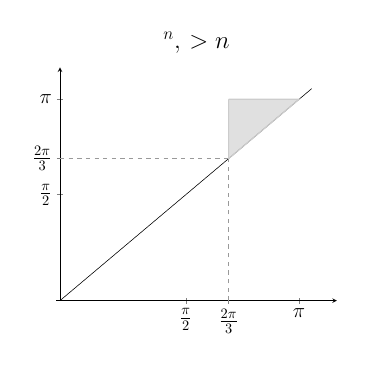
\begin{tikzpicture}[scale=0.52]
	\begin{axis} [
		title={\LARGE $\Hbarc{\degp}{\rp^n},\, \degp>n$},
		ticklabel style = {font=\Large},
		axis y line=middle,
		axis x line=middle,
		ytick={0.5,0.67,0.95},
		yticklabels={$\frac{\pi}{2}$,$\frac{2\pi}{3}$,$\pi$},
		xtick={0.5,0.67,0.95},
		xticklabels={$\frac{\pi}{2}$,$\frac{2\pi}{3}$,$\pi$},
		xmin=-0.015, xmax=1.1,
		ymin=0, ymax=1.1,]
		\addplot [mark=none] coordinates {(0,0) (1,1)};
		\addplot [thick,color=black!20!white,fill=black!30!white,
		fill opacity=0.4]coordinates {
			(0.67,0.95)
			(0.67,0.67)
			(0.95,0.95)
			(0.67,0.95)};
		\addplot [black!40!white,mark=none,dashed, thin] coordinates {(0,0.67) (0.67,0.67)};
		\addplot [black!40!white,mark=none,dashed, thin] coordinates {(0.67,0) (0.67,0.67)};
		% \addplot[barccolor,mark=*] (0, 0.67) circle (2pt) node[above right,barccolor]{\Large\textsf{1}};
		% \node[mark=none] at (axis cs:0.68,0.21){$\Hbarc{\degp}{\rp^n},\, \degp\geq 2$};
	\end{axis}
\end{tikzpicture}

\begin{tikzpicture}[scale=0.52]
	\begin{axis} [
		title = {\LARGE $\sqbarcl{k}{}{\rp^n},\, m \leq n$ and $\binom{m-k}{k}$ odd},
		ticklabel style = {font=\Large},
		axis y line=middle,
		axis x line=middle,
		ytick={0.5,0.67,0.95},
		yticklabels={$\frac{\pi}{2}$,$\frac{2\pi}{3}$,$\pi$},
		xtick={0.5,0.67,0.95},
		xticklabels={$\frac{\pi}{2}$,$\frac{2\pi}{3}$,$\pi$},
		xmin=-0.015, xmax=1.1,
		ymin=0, ymax=1.1,]
		\addplot [mark=none] coordinates {(0,0) (1,1)};
		\addplot [thick,color=black!20!white,fill=black!30!white,
		fill opacity=0.4]coordinates {
			(0.67,0.95)
			(0.67,0.67)
			(0.95,0.95)
			(0.67,0.95)};
		\addplot [black!40!white,mark=none,dashed, thin] coordinates {(0,0.67) (0.67,0.67)};
		%\addplot [black!40!white,mark=none,dashed, thin] coordinates {(0,0.72) (0.72,0.72)};
		\addplot [black!40!white,mark=none,dashed, thin] coordinates {(0.67,0) (0.67,0.67)};
		\addplot[barccolor,mark=*] (0, 0.67) circle (2pt) node[above right,barccolor]{};
        %{\Large$\geq$\textsf{1}};
	\end{axis}
\end{tikzpicture}
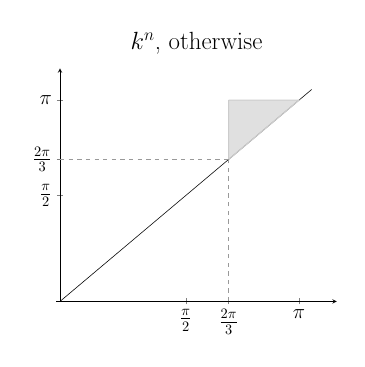
\begin{tikzpicture}[scale=0.52]
	\begin{axis} [
		title={\LARGE $\sqbarcl{k}{}{\rp^n}$, otherwise},
		ticklabel style = {font=\Large},
		axis y line=middle,
		axis x line=middle,
		ytick={0.5,0.67,0.95},
		yticklabels={$\frac{\pi}{2}$,$\frac{2\pi}{3}$,$\pi$},
		xtick={0.5,0.67,0.95},
		xticklabels={$\frac{\pi}{2}$,$\frac{2\pi}{3}$,$\pi$},
		xmin=-0.015, xmax=1.1,
		ymin=0, ymax=1.1,]
		\addplot [mark=none] coordinates {(0,0) (1,1)};
		\addplot [thick,color=black!20!white,fill=black!30!white,
		fill opacity=0.4]coordinates {
			(0.67,0.95)
			(0.67,0.67)
			(0.95,0.95)
			(0.67,0.95)};
		\addplot [black!40!white,mark=none,dashed, thin] coordinates {(0,0.67) (0.67,0.67)};
		\addplot [black!40!white,mark=none,dashed, thin] coordinates {(0.67,0) (0.67,0.67)};
	\end{axis}
\end{tikzpicture}
	\caption{\emph{Top row:} the $\degp^\th$ persistent homology barcode of $\rp^n$.
		When $1\leq \degp \leq n$, the barcode consists of one $(0,\frac{2\pi}{3})$ and potentially some bars dominated by $(\frac{2\pi}{3}, \pi)$.
		\emph{Bottom row:} the degree-$(k+\ell)$ component of the $\Sq^k$-barcode of $\rp^n$.
		The leftmost barcode contains at least one $(0,\gamma_m)$ and potentially some bars dominated by $(\frac{2\pi}{3}, \pi)$.
		See \cref{sub:barcode_rpn}.
	}
	\label{fig:sq barcodes}
\end{figure}


\section{Gromov--Hausdorff estimates}\label{prop:db estimate}

We estimate the bottleneck distance $\db$ between the Steenrod barcodes of certain pairs of metric spaces and demonstrate that it provides a tighter lower-bound approximation of the Gromov–Hausdorff distance between the spaces than $\db$ between their persistent homology barcodes.
See the theorem in \cref{subsub:main_theorem} for details.
Although this theorem is stated for $\bS^1\vee\dots\vee \bS^n$ and $\rp^n$ only, we present our methodology within a more general framework.
This allows us to identify the essential components of the proof, laying the groundwork for extending these results to other spaces.

Let $\cX$ be a totally bounded metric space of diameter $\pi$, where the first critical value $\alpha$ of $\VR\cX$ satisfies $\alpha \geq \zeta_n = \arccos{(-\tfrac{1}{n+1})}$ and $n$ is the largest degree such that the $n^\th$ reduced homology of $\cX$ is non-trivial.
Let $\VS \defeq \VS^{\ell_1, \dots, \ell_n}$ with $\ell_i = \dim \opH_i(\cX)$ for each $i=1, \dots, n$.

Let $\beta_\degp$ and $\gamma_\degp$ denote the first critical values of the $\degp^\th$ reduced homology of $\VR\cX$ and the degree-$\degp$ component of the $\theta$-barcode of $\VR\cX$, respectively.

\subsection{Upper bound on $\db$ between homology barcodes}
\label{subsub:db_upper_bound}

To obtain an upper bound on the bottleneck distance, it suffices to find one matching and compute the cost of it.

\medskip\proposition
For any degree $\degp$ such that $\opH_\degp(\cX)$ is non-trivial,
\begin{equation}\label{eq:db_usual_upper_bound}
	\db(\Hbarc[\field]{\degp}{\VS}, \Hbarc[\field]{\degp}{\cX})
	%\leq \cost(P)
	\leq \max\{|\zeta_\degp  - \beta_\degp |, \tfrac{\pi - \zeta_n}{2}\}.
\end{equation}

\begin{proof}
	Consider the matching $P$ between $\Hbarc[\field]{\degp}{\VS}$ and $\Hbarc[\field]{\degp}{\cX}$ such that $(0,\zeta_\degp ) \leftrightarrow (0, \beta_\degp )$ and all other bars unmatched.
	Using the barcode estimates \cref{fig:barcodes_vs} and \cref{fig:barcodes_general}, we obtain that the cost of $P$ satisfies
	\begin{align*}
		\cost(P)
		= & \max\{|\zeta_\degp  - \beta_\degp |, \tfrac{\pi - \zeta_n}{2}, \tfrac{\pi - \alpha}{2}\} \\
		= & \max\{|\zeta_\degp  - \beta_\degp |, \tfrac{\pi - \zeta_n}{2}\} && \mbox{(because $\zeta_n \leq \alpha$)}.
	\end{align*}
	Therefore, \cref{eq:db_usual_upper_bound} holds.
\end{proof}


% For any degree $m > n$, consider the matching $P$ between $\Hbarc[\field]{\degp}{\VS}$ and $\Hbarc{\degp}{\cX}$ such that all bars are unmatched. Then the cost of $P$ satisfies:
% \[
%     \cost(P)
%     = \max\{\tfrac{\pi - \zeta_n}{2}, \tfrac{\pi - \alpha}{2}\}
%     = \tfrac{\pi - \zeta_n}{2}.
% \]

\subsection{Lower bound on $\db$ between $\theta$-barcodes}
\label{subsub:db_theta_lower_bound}

To obtain a lower bound on the bottleneck distance, the minimum cost of matching a certain bar is calculated.

\medskip\proposition
Let $\theta \in \cO(\ell, \degp)$ be a linear cohomology operation such that $\img \theta_\cX$ is non-trivial.
Then,
\begin{equation}\label{eq:db_theta_lower_bound}
	\db(\thetabarc{\VS}, \thetabarc{\cX})
	%= \min_Q \cost(Q)
	\geq \min\{\tfrac{\gamma_\degp }{2}, \zeta_n\}. %\geq \tfrac{\zeta_n}{2}.
\end{equation}

\begin{proof}
	Recall from \cref{fig:barcodes_general} that $\thetabarc{\cX}$ contains a bar $(0,\gamma_\degp)$.
	We calculate the minimum cost of matching the bar $(0,\gamma_\degp)$.

	Let $Q$ be an arbitrary matching between $\thetabarc{\VS}$ and $\thetabarc{\cX}$.
	If $(0,\gamma_\degp )$ is unmatched in $Q$, then $\cost(Q) \geq \tfrac{\gamma_\degp }{2}$.
	If $(0,\gamma_\degp )$ is matched to some bar $(a,b) \subset (\zeta_n, \pi)$ in $\thetabarc{\VS}$ in $Q$, then
	$\cost(Q) =  \|(0,\gamma_\degp ) - (a,b)\|_\infty \geq \zeta_n$.
	Thus, an arbitrary matching $Q$ between $\thetabarc{\VS}$ and $\thetabarc{\cX}$ must satisfy $\cost(Q) \geq \min\{\tfrac{\gamma_\degp }{2}, \zeta_n\}.$
	Therefore, \cref{eq:db_theta_lower_bound} holds.
\end{proof}

\subsection{Technical lemma}
\label{subsub:comparison_lemma}

We establish a technical lemma.

\medskip\lemma
\begin{itemize}
	\item If $\beta_\degp \in [\alpha, \tfrac{\pi - \zeta_n}{2}+\zeta_\degp]$, then
	$\max\{|\zeta_\degp  - \beta_\degp |, \tfrac{\pi - \zeta_n}{2}\}
	\leq \tfrac{\pi - \zeta_n}{2}$.
	\item If $\beta_\degp \in (\tfrac{\pi - \zeta_n}{2}+\zeta_\degp, \tfrac{\zeta_n}{2}+\zeta_\degp)$, then
	$\max\{|\zeta_\degp  - \beta_\degp |, \tfrac{\pi - \zeta_n}{2}\}
	\leq \tfrac{\zeta_n}{2}$.
\end{itemize}

\begin{proof}
	First consider when $\beta_\degp \in [\alpha, \tfrac{\pi - \zeta_n}{2}+\zeta_\degp]$ and divide the discussion to two cases.
	If $\beta_\degp \leq \zeta_\degp$, then because $\tfrac{\pi}{2} < \alpha \leq \beta_\degp \leq \zeta_\degp  \leq \tfrac{2\pi}{3}$ and $\zeta_n \leq \tfrac{2\pi}{3}$, we have
	\[
	|\zeta_\degp  - \beta_\degp |
	= \zeta_\degp  - \beta_\degp
	< \tfrac{2\pi}{3} - \tfrac{\pi}{2}
	= \tfrac{\pi}{6}
	\leq \tfrac{\pi - \zeta_n}{2}.
	\]
	If $\beta_\degp > \zeta_\degp$, then
	\[
	|\zeta_\degp  - \beta_\degp |
	= \beta_\degp - \zeta_\degp
	\leq \tfrac{\pi - \zeta_n}{2} + \zeta_\degp - \zeta_\degp
	= \tfrac{\pi - \zeta_n}{2}.
	\]
	Thus, $\max\{|\zeta_\degp  - \beta_\degp |, \tfrac{\pi - \zeta_n}{2}\} = \tfrac{\pi - \zeta_n}{2}.$

	When $\beta_\degp \in (\tfrac{\pi - \zeta_n}{2}+\zeta_\degp, \tfrac{\zeta_n}{2}+\zeta_\degp)$, we have
	\[
	\max\{|\zeta_\degp  - \beta_\degp |, \tfrac{\pi - \zeta_n}{2}\}
	= \max\{\beta_\degp - \zeta_\degp, \tfrac{\pi - \zeta_n}{2}\}
	< \max\{\tfrac{\zeta_n}{2}+\zeta_\degp - \zeta_\degp, \tfrac{\pi - \zeta_n}{2}\}
	= \tfrac{\zeta_n}{2} .
	\]
\end{proof}

\subsection{Comparison}
\label{subsub:main_theorem}

\subsubsection{}
By combining results from \cref{subsub:db_upper_bound}, \cref{subsub:db_theta_lower_bound} and \cref{subsub:comparison_lemma}, we immediately obtain that the lower bound of the bottleneck distance $\db$ between the $\theta$-barcodes of the two space $\VS$ and $\cX$ (Equation (\ref{eq:db_theta_lower_bound})) is larger than the upper bound of $\db$ between the persistent homology barcodes of the two spaces (Equation (\ref{eq:db_usual_upper_bound})).
As a consequence, the $\theta$-barcodes provide a better (lower-bound) approximation of the Gromov--Hausdorff distance than $\db$ between the persistent homology barcodes.

\medskip\proposition

If $\theta \in \cO(\ell, \degp)$ is a linear cohomology operation such that $\img \theta_\cX$ is non-trivial, then
\[\db(\thetabarc{\VS}, \thetabarc{\cX}) \geq \db(\Hbarc[\field]{\degp}{\VS}, \Hbarc[\field]{\degp}{\cX}).\]

\subsubsection{}

In the case of $\cX = \rp^n$ and the cohomology operations $\theta$ being the Steenrod squares, all with mod $2$ coefficients, we have a finer estimate as in the theorem below.
Below, $\VS$ is $\bS^1\vee\dots\vee \bS^n$.

\medskip\theorem
We have
\begin{itemize}
	\item[(a)] $\max_{\degp\geq 1}\db(\Hbarc{\degp}{\VS}, \Hbarc{\degp}{\rp^n})\leq \tfrac{\pi - \zeta_n}{2}$.
	\smallskip\item[(b)] $\db(\sqbarcl{k}{\ell}{\VS}, \sqbarcl{k}{\ell}{\rp^n})\geq \tfrac{\pi}{3}$, for $k,\ell$ such that $1\leq k \leq \frac{n-1}{2}$ and $\binom{\ell}{k} \mod 2 \neq 0$.
\end{itemize}

\begin{proof}
	As shown in \cref{sub:first_critical_value_rpn}, the first critical values satisfy
	$$
	\alpha = \beta_\degp = \gamma_{k+\ell} = \frac{2\pi}{3}
	$$
	for any $1 \leq \degp \leq n$, and $k$ and $\ell$ such that $1\leq k \leq \frac{n-1}{2}$ and $\binom{\ell}{k} \mod 2 \neq 0$.
	It is clear that $\alpha= \tfrac{2\pi}{3}$ lies in $[\zeta_n, \pi)$ and $\beta_\degp = \tfrac{2\pi}{3}$ lies in $[\alpha, \tfrac{\pi - \zeta_n}{2}+\zeta_\degp]$ satisfying the first condition of the lemma in \cref{subsub:comparison_lemma}.
	It follows from \cref{eq:db_usual_upper_bound} and \cref{subsub:comparison_lemma} that
	\[\max_{\degp\geq 1}\db(\Hbarc{\degp}{\VS}, \Hbarc{\degp}{\rp^n})\leq \tfrac{\pi - \zeta_n}{2}.\]

	We have shown in \cref{subsub:first_critical_value} that the first critical value $\gamma_{\ell+k}$ is $\tfrac{2\pi}{3}$.
	Applying \cref{eq:db_theta_lower_bound}, we have
	\[\db(\sqbarcl{k}{\ell}{\VS}, \sqbarcl{k}{\ell}{\rp^n})
	\geq \min\{\tfrac{\gamma_{\ell+k}}{2}, \zeta_n\}
	= \min\{\tfrac{1}{2}\cdot\tfrac{2\pi}{3}, \zeta_n\}
	= \tfrac{\pi}{3}.\]
\end{proof}

Because $\tfrac{\pi}{3} < (\tfrac{\pi}{4} <) \tfrac{\pi - \zeta_n}{2}$, the above theorem shows that the Steenrod barcodes provide a better lower bound estimate of the Gromov--Hausdorff distance than the persistent homology barcodes do in all degrees.
